\documentclass{beamer}
\mode<presentation>
\usepackage{amsmath,amssymb,mathtools}
\usepackage{textcomp}
\usepackage{gensymb}
\usepackage{adjustbox}
\usepackage{subcaption}
\usepackage{enumitem}
\usepackage{multicol}
\usepackage{listings}
\usepackage{url}
\usepackage{graphicx} % <-- needed for images
\def\UrlBreaks{\do\/\do-}

\usetheme{Boadilla}
\usecolortheme{lily}
\setbeamertemplate{footline}{
  \leavevmode%
  \hbox{%
  \begin{beamercolorbox}[wd=\paperwidth,ht=2ex,dp=1ex,right]{author in head/foot}%
    \insertframenumber{} / \inserttotalframenumber\hspace*{2ex}
  \end{beamercolorbox}}%
  \vskip0pt%
}
\setbeamertemplate{navigation symbols}{}

\lstset{
  frame=single,
  breaklines=true,
  columns=fullflexible,
  basicstyle=\ttfamily\tiny   % tiny font so code fits
}

\numberwithin{equation}{section}

% ---- your macros ----
\providecommand{\brak}[1]{\ensuremath{\left(#1\right)}}
\providecommand{\myvec}[1]{\ensuremath{\begin{pmatrix}#1\end{pmatrix}}}
\providecommand{\norm}[1]{\lVert#1\rVert}

\title{Matgeo Presentation - Direction Cosines Problem}
\author{EE25BTECH11048 - Revanth Siva Kumar D}

\begin{document}

\begin{frame}
  \titlepage
\end{frame}

\begin{frame}{Problem Statement}
\textbf{Question:}  

If the direction cosines of a line are $\brak{k,k,k}$, then find the value of $k$.\\

\textbf{Goal:} Determine $k$ and visualize the direction vectors in 3D.
\end{frame}

\begin{frame}{Theoretical Solution}
The direction cosines of a line are denoted by $k, k, k$.  
So, the direction cosine vector becomes
\begin{align}
\vec{d} = \myvec{k \\ k \\ k}
\label{eq:dc_condition}
\end{align}
since d is a unit vector \begin{align}
    \norm{d}=1
    \label{eq:norm}
\end{align}

Applying condition \eqref{eq:dc_condition},
\begin{align}
(from \eqref{eq:norm} \norm{d}=1)\\
\norm{\myvec{k\\k\\k}} &= 1\\
\sqrt{3k^2} &= 1 \\ 
3k^2 &= 1 \implies k^2=\frac{1}{3}
\end{align}
\end{frame}
\begin{frame}{Theoretical Solution}
Hence,
\begin{align}
k = \pm \frac{1}{\sqrt{3}}
\end{align}

So, the line vectors are
\[
\vec{v}_1 = \myvec{\frac{1}{\sqrt{3}} \\ \frac{1}{\sqrt{3}} \\ \frac{1}{\sqrt{3}}}, 
\quad
\vec{v}_2 = \myvec{-\frac{1}{\sqrt{3}} \\ -\frac{1}{\sqrt{3}} \\ -\frac{1}{\sqrt{3}}}
\]

\textbf{Answer:} 
\[
k = \frac{1}{\sqrt{3}} \quad \text{or} \quad k = -\frac{1}{\sqrt{3}}
\]
\end{frame}

\section*{Appendix: Code}

\begin{frame}[fragile]{C Code: points.c}
\begin{lstlisting}[language=C]
#include <math.h>
#include <stdio.h>

// Function to compute direction cosine k
// Returns positive root; negative handled in Python
double compute_k() {
    double k = 1.0 / sqrt(3.0);
    return k;
}

int main() {
    double k = compute_k();
    printf("k = %lf\n", k);
    printf("-k = %lf\n", -k);
    return 0;
}
\end{lstlisting}
\end{frame}

\begin{frame}[fragile]{Python: call\_c.py}
\begin{lstlisting}[language=Python]
import ctypes
import numpy as np
import matplotlib.pyplot as plt
from mpl_toolkits.mplot3d import Axes3D

# Load shared object
lib = ctypes.CDLL("./points.so")
lib.compute_k.restype = ctypes.c_double

# Call C function to get positive k
k_pos = lib.compute_k()
k_neg = -k_pos

print("Possible values of k from C: k =", k_pos, "or", k_neg)

# Vectors for plotting
vec_pos = np.array([k_pos, k_pos, k_pos])
vec_neg = np.array([k_neg, k_neg, k_neg])
\end{lstlisting}
\end{frame}
\begin{frame}[fragile]{Python: call\_c.py}
\begin{lstlisting}[language=Python]
# 3D plot
fig = plt.figure()
ax = fig.add_subplot(111, projection='3d')
origin = np.array([0,0,0])

# Plot both vectors
ax.quiver(*origin, *vec_pos, color='r', arrow_length_ratio=0.1,
          label=f"(k,k,k), k={k_pos:.3f}")
ax.quiver(*origin, *vec_neg, color='b', arrow_length_ratio=0.1,
          label=f"(-k,-k,-k), k={k_pos:.3f}")

ax.set_xlim([-0.7,0.7])
ax.set_ylim([-0.7,0.7])
ax.set_zlim([-0.7,0.7])

ax.set_xlabel("X")
ax.set_ylabel("Y")
ax.set_zlabel("Z")
ax.set_title("Direction Cosine Vectors from C")
ax.legend()
plt.show()
\end{lstlisting}
\end{frame}

\begin{frame}{3D Plot of Direction Cosines}
\begin{figure}[h!]
  \centering
  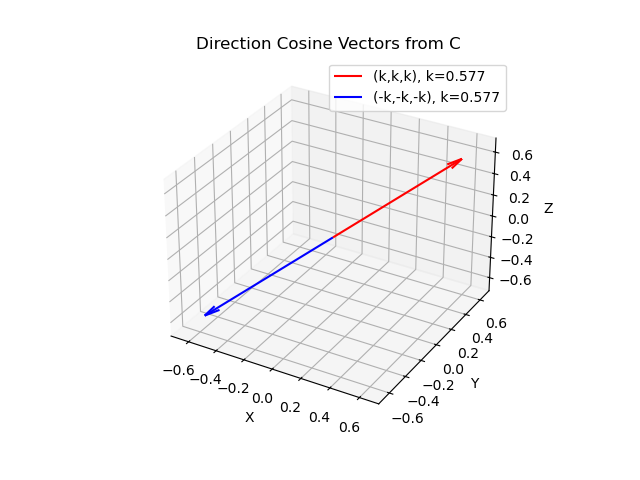
\includegraphics[width=0.6\columnwidth]{figs/Figure_1.png} 
   \caption*{3D plot of direction cosine vectors $(k,k,k)$ and $(-k,-k,-k)$ using shared output}
   \label{Fig:dircosines}
\end{figure}
\end{frame}
\begin{frame}[fragile]{Python: plot.py}
\begin{lstlisting}[language=Python]
import numpy as np
import matplotlib.pyplot as plt
from mpl_toolkits.mplot3d import Axes3D

# Direction cosine values
k1 = 1 / np.sqrt(3)
k2 = -k1

print("Possible values: k =", k1, "or", k2)

# Vectors for plotting
vec_pos = np.array([k1, k1, k1])
vec_neg = np.array([k2, k2, k2])

fig = plt.figure()
ax = fig.add_subplot(111, projection='3d')
origin = np.array([0,0,0])
\end{lstlisting}
\end{frame}
\begin{frame}[fragile]{Python: plot.py}
\begin{lstlisting}[language=Python]
# Plot both vectors
ax.quiver(*origin, *vec_pos, color='g', arrow_length_ratio=0.1,
          label=f"(k,k,k), k={k1:.3f}")
ax.quiver(*origin, *vec_neg, color='r', arrow_length_ratio=0.1,
          label=f"(-k,-k,-k), k={k1:.3f}")

ax.set_xlim([-0.7,0.7])
ax.set_ylim([-0.7,0.7])
ax.set_zlim([-0.7,0.7])

ax.set_xlabel("X")
ax.set_ylabel("Y")
ax.set_zlabel("Z")
ax.set_title("Direction Cosine Vectors")
ax.legend()
plt.savefig("dir_cosines_both.png")
plt.show()
\end{lstlisting}
\end{frame}
\begin{frame}{3D Plot of Direction Cosines}

\begin{figure}[h!]
  \centering
  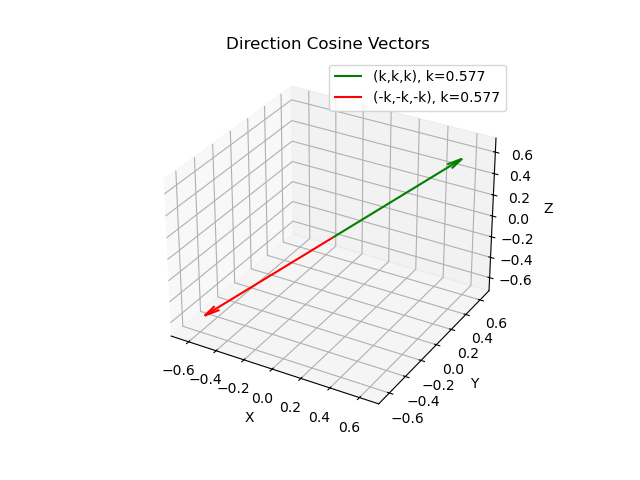
\includegraphics[width=0.6\columnwidth]{figs/Figure_2.png} 
   \caption*{3D plot of direction cosine vectors $(k,k,k)$ and $(-k,-k,-k)$ by direct python code}
   \label{Fig:dircosines}
\end{figure}
    
\end{frame}
\end{document}



